\documentclass[11pt]{beamer}
%\documentclass[handout,dvips,11pt,grey]{beamer}

\usepackage{multicol}
\usepackage{verbatim}
\usepackage{graphicx}
\usepackage{listings}

% ``define'' Scala
\lstdefinelanguage{scala}{
  morekeywords={abstract,case,catch,class,def,%
    do,else,extends,false,final,finally,%
    for,if,implicit,import,match,mixin,%
    new,null,object,override,package,%
    private,protected,requires,return,sealed,%
    super,this,throw,trait,true,try,%
    type,val,var,while,with,yield},
  otherkeywords={=>,<-,<\%,<:,>:,\#,@},
  sensitive=true,
  morecomment=[l]{//},
  morecomment=[n]{/*}{*/},
  morestring=[b]'',
  morestring=[b]',
  morestring=[b]"''
}
\usepackage{hyperref}

\begin{document}

\title{PPAML2015 Summer School}

\subtitle{Geolocation Using Wi-Fi Signal in Figaro}

\author{Sebastian Imlay, Daniel Salvadori, Philip M. Robinson}

\institute{PPAML}

\date{\today}

\begin{frame}
  \titlepage
\end{frame}


\begin{frame}{Domain Problem}

\end{frame}

\begin{frame}{Model Discussion and History}
\begin{center}
\begin{multicols}{3}
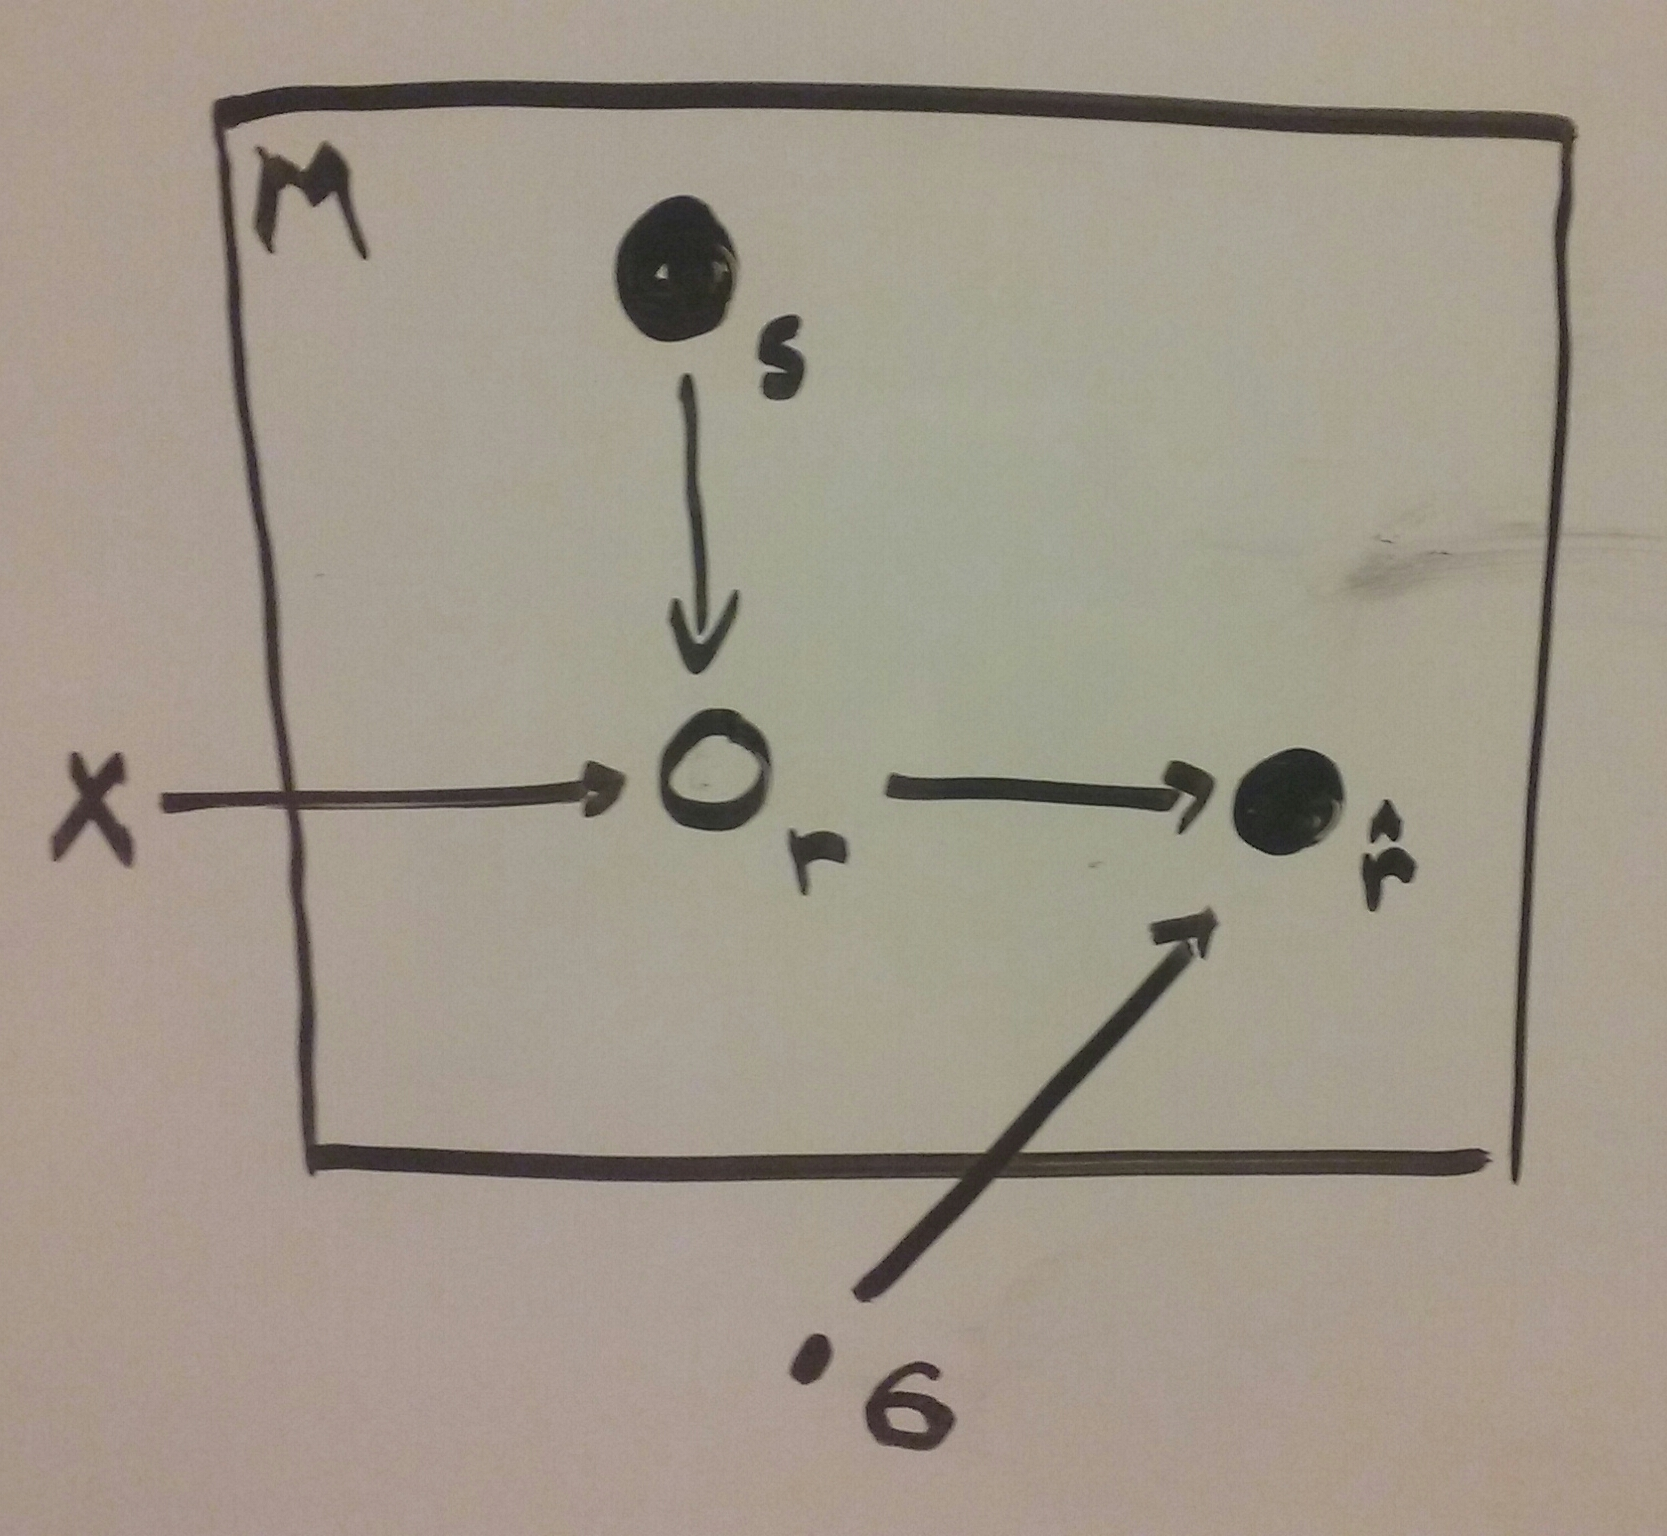
\includegraphics[height=1in]{pictures/1plate.jpg}

%abcd
\columnbreak

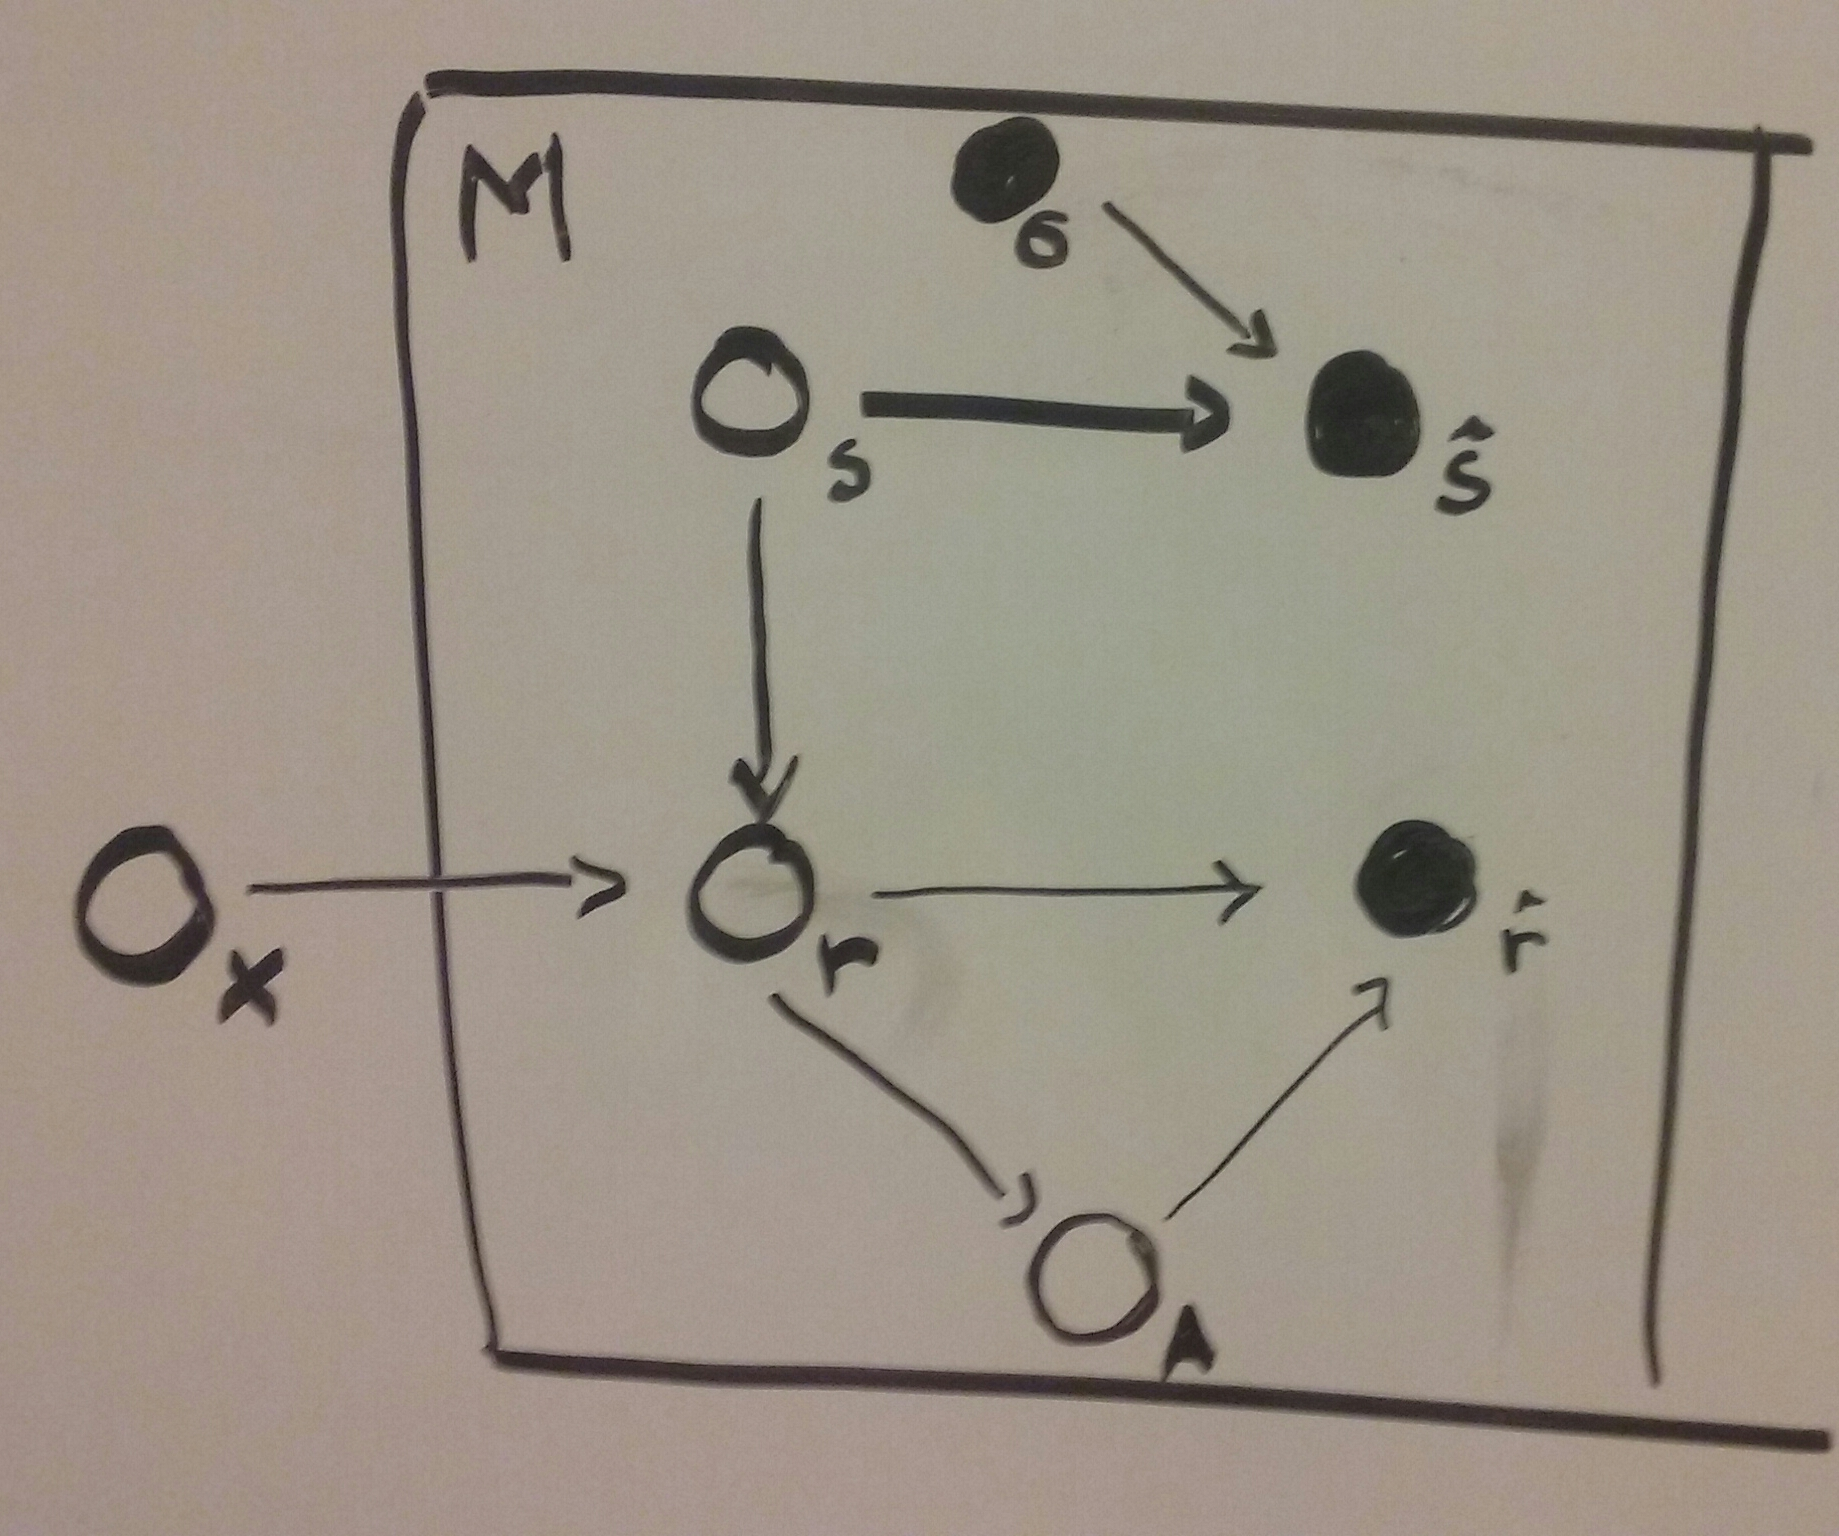
\includegraphics[height=1in]{pictures/2plate.jpg}

%abcd
\columnbreak

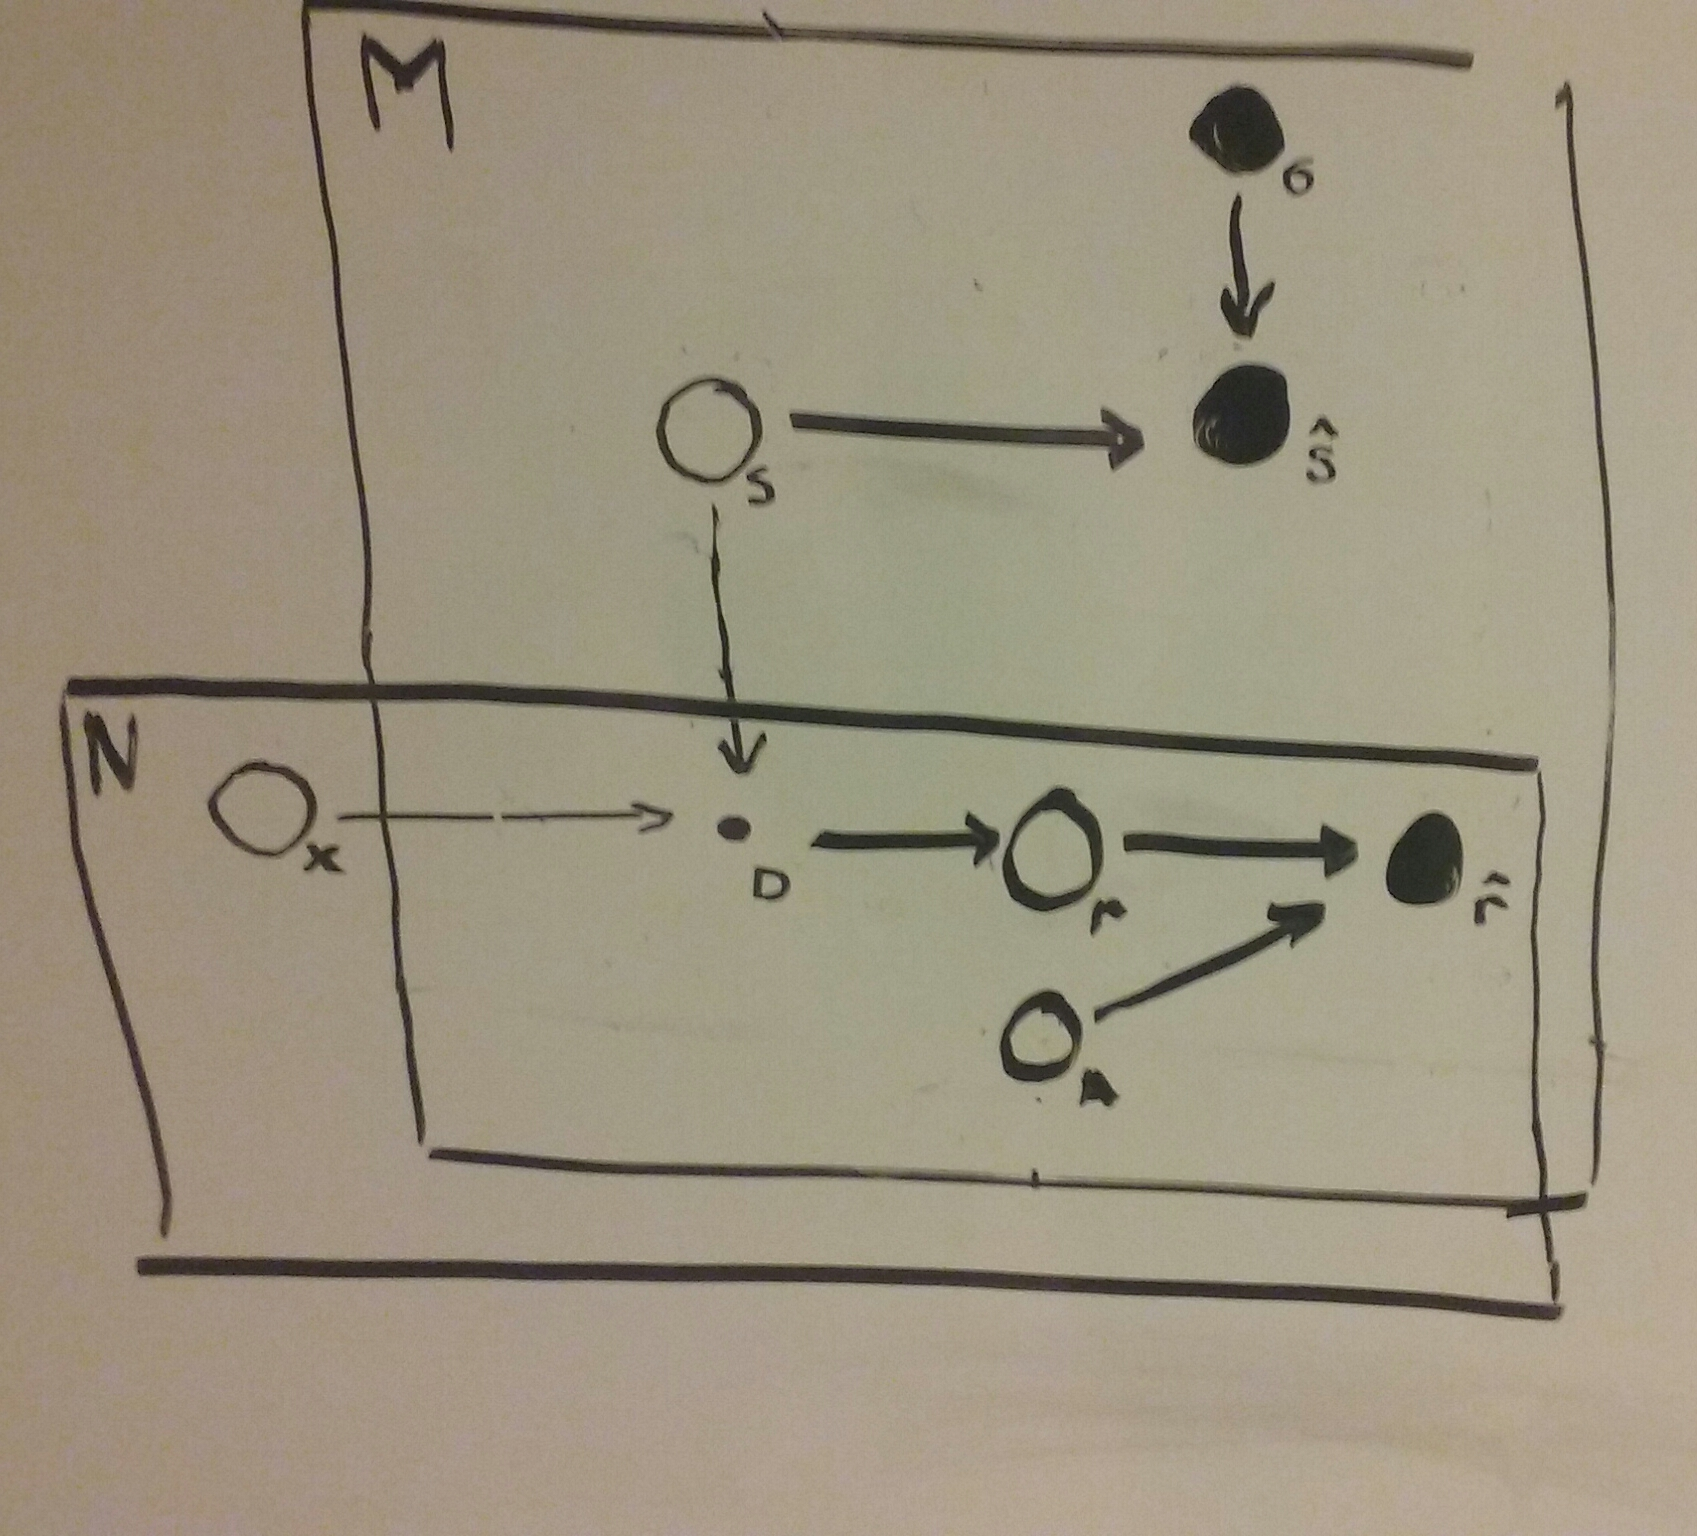
\includegraphics[height=1in]{pictures/3plate.jpg}

%abcd
\columnbreak
\end{multicols}
\end{center}
\begin{itemize}
\item[N] Transmitters
\item[M] Receivers
\item[S] Receiver Position
\item[X] Receiver Position
\item[r] Power
\item[A] Attenuation
\item[D] Distance
\end{itemize}

\end{frame}

\begin{frame}{Implementation - Supporting Technology}

    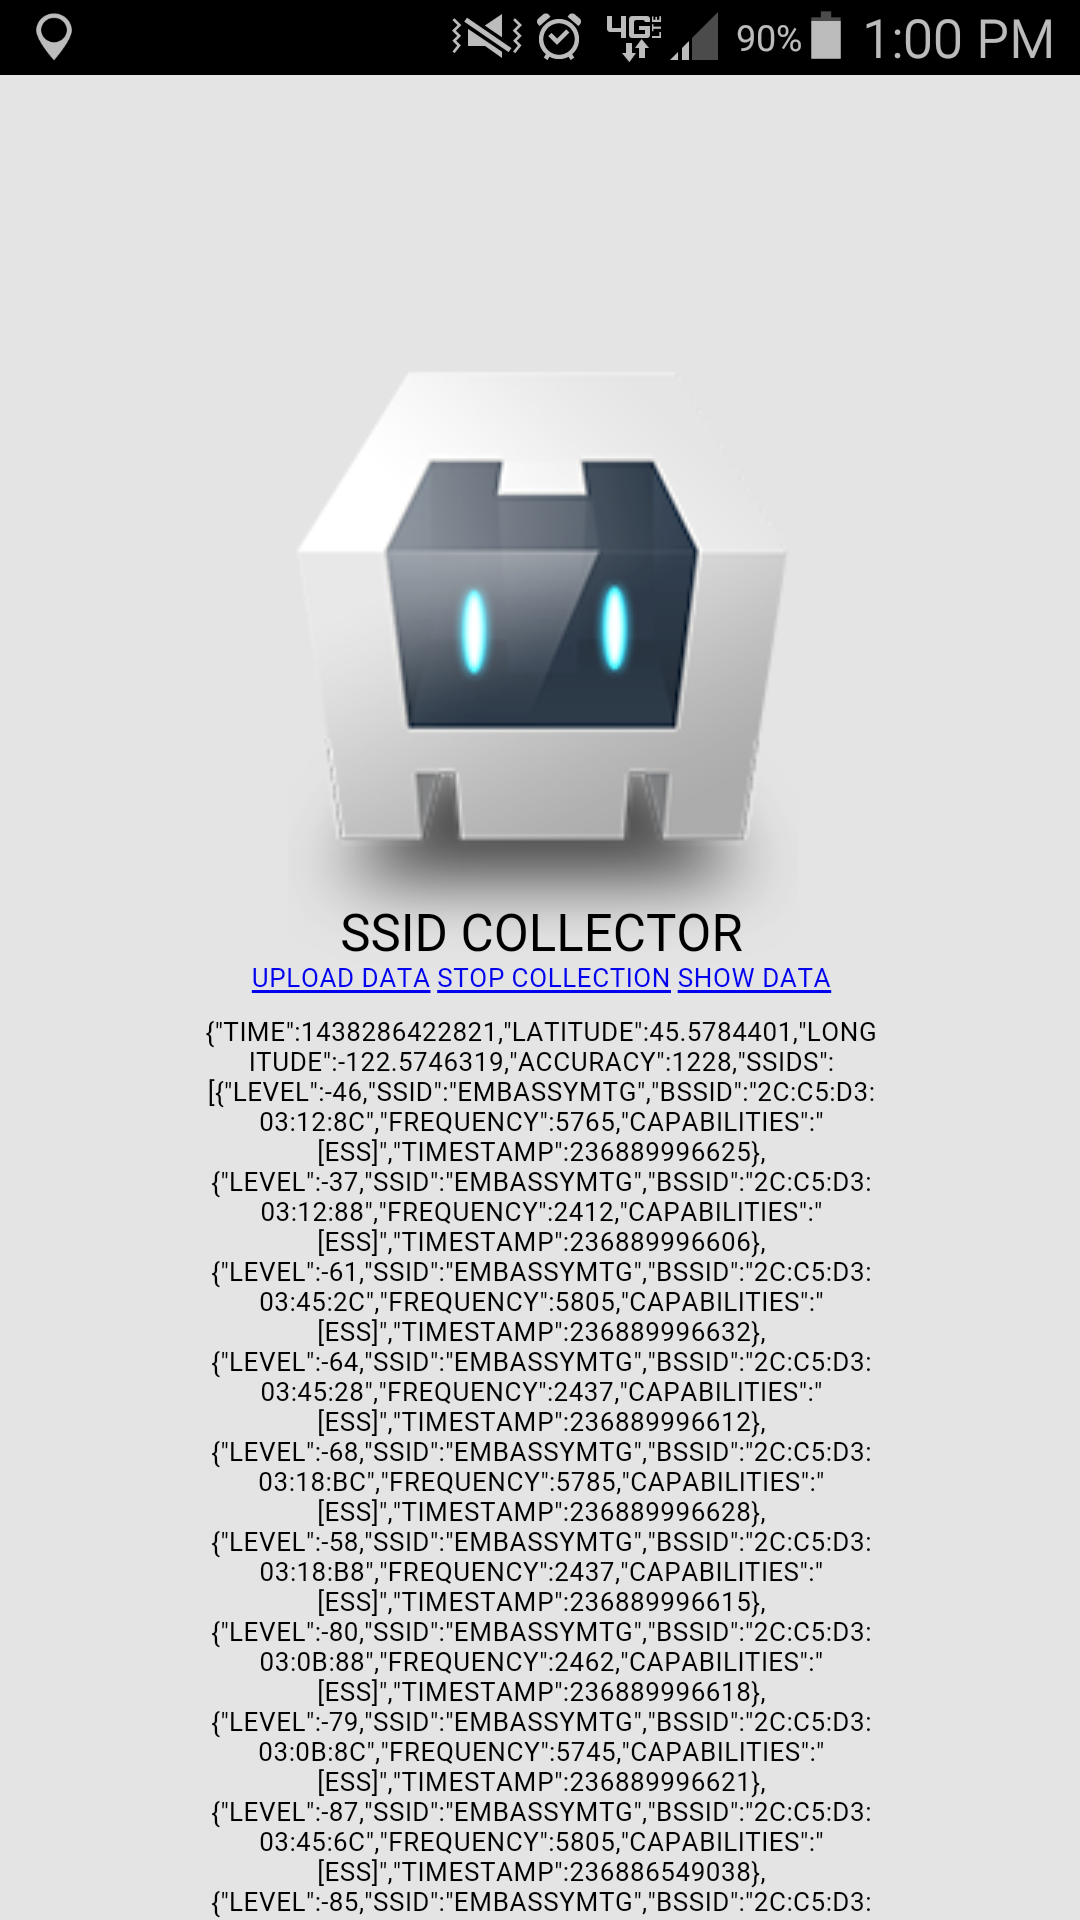
\includegraphics[height=0.7\textheight]{pictures/phoneapp.png}
    \begin{itemize}
        \item Phone app - Apache Cordova
        \item Backend - Couchdb
    \end{itemize}

\end{frame}

\begin{frame}{Interactive Visualization}

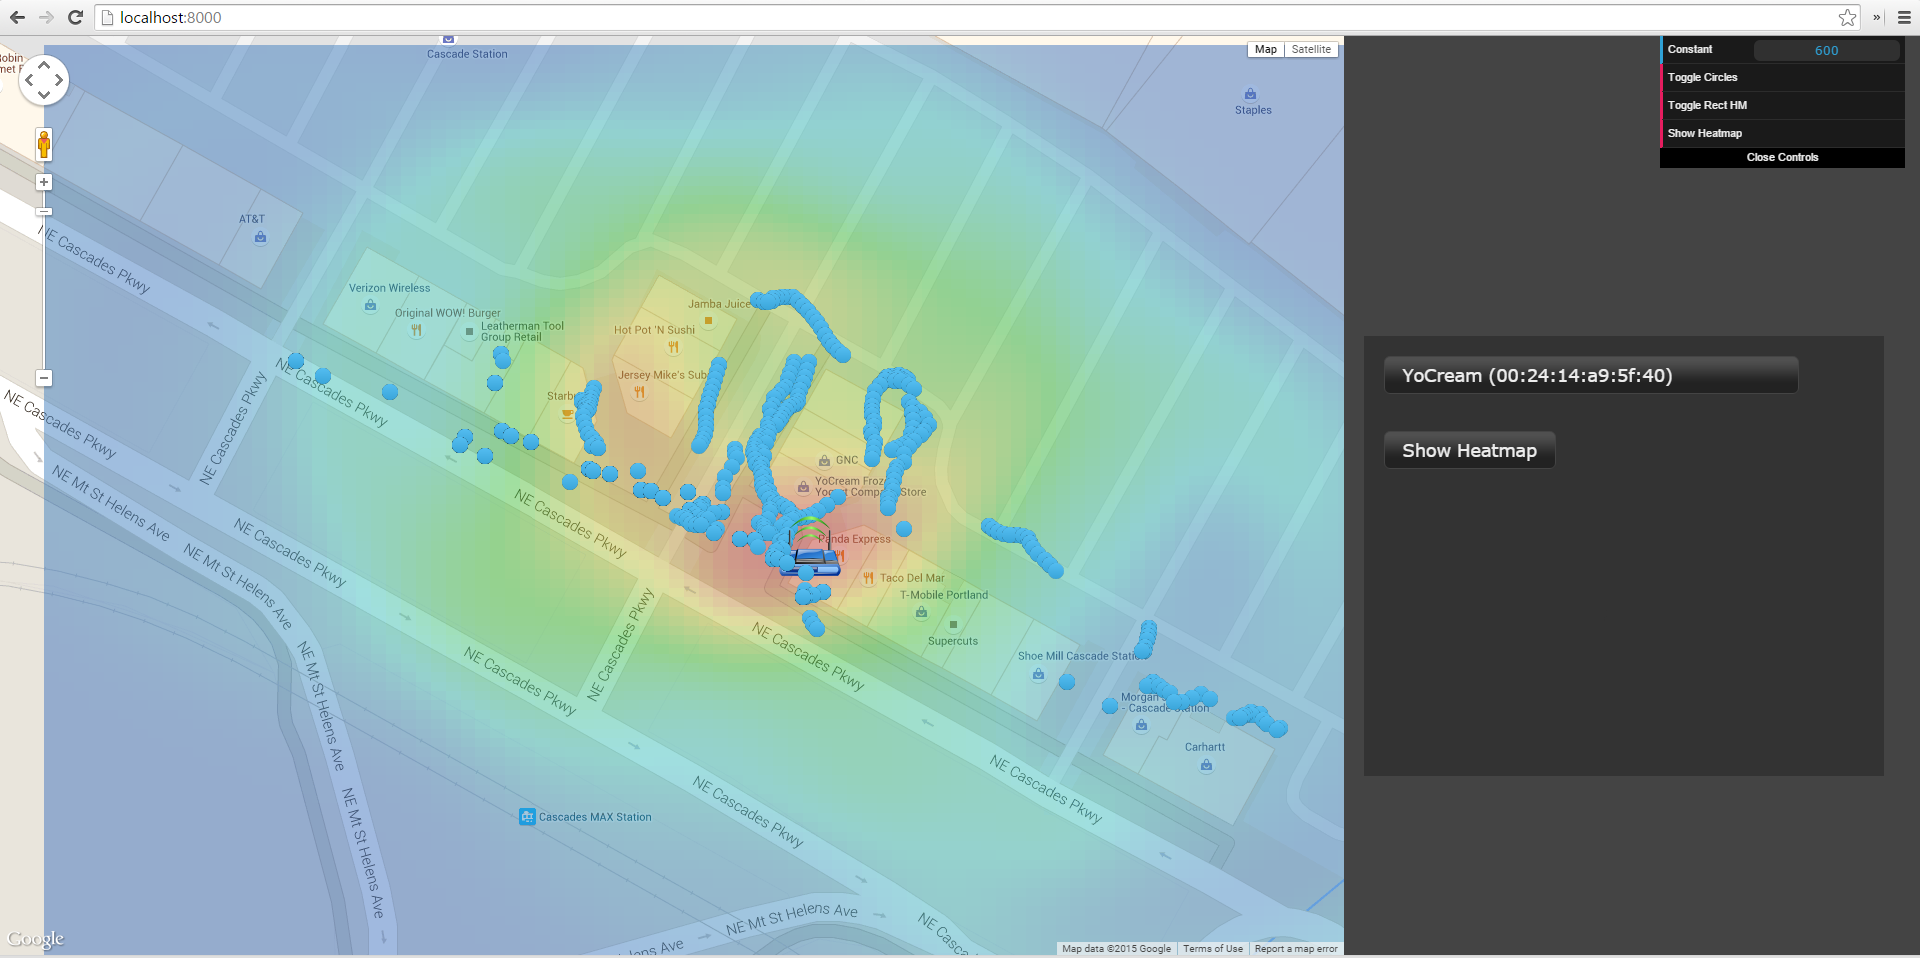
\includegraphics[height=0.55\textheight]{pictures/screenshot4.png}

\href{http://localhost:8000/}{Interactive Visualization Demo}

\end{frame}

\begin{frame}{Implementation - Figaro}
\begin{multicols}{2}
\resizebox{!}{1.5in}{\lstinputlisting[
    basicstyle=\footnotesize,
    numbers=left,
    numberstyle=\tiny\color{gray}
  ]{probinso.scala}
}
\columnbreak

\begin{itemize}
\item We all implented our own version of the solution in figaro, and used eachothers solutions to guide us when we got stuck
\item Fist pass we were writing procedural solutions, and our programs didn't really make sence
\item Identifying smaller models, and sculpting data to fit those models helped us think about our problem space
\end{itemize}
\end{multicols}

\end{frame}

\begin{frame}{Insights}

\end{frame}

\begin{frame}{Collateral}

\end{frame}

\end{document}
